\documentclass[11pt]{article}
\usepackage{float}
\usepackage{graphicx}
%Gummi|065|=)
\title{\textbf{Interactive Vizualization}
\\
\normalsize{Assigment 2}
}
\author{Ian Ooi\\
		Max Espinoza}
\begin{document}

\maketitle


\section{Discussion of Results}

The easiest graph to implement was a general undirected graph. VTK uses layout strategies to control how those nodes where displayed. Some are familiar in that they include strategies such as forced-directed, clustering, and randomly assigned 2d layout. While these were great to start to visualizes inputs quickly, it actually provided difficult when we wanted to implement our own strategy or modify existing ones. Visualizing a clique, disconnected graph, non planar graphs were easy. However trying to implement trees, planar graphs, and bipartite graphs proved a challenge because we had to dig deeply into implementation of VTK to control where vertices's were being placed. I couldn't have done better by hand, so I can't complain, I do wish that the tool offered more control or documentation on the underlying data structures and how to use them to generate new 2D layouts strategies.



\section{Review Of VTK}

    VTK has a very poor community presence and only moderate presence online, which makes getting started and continuing with the tool very difficult.  It has a fairly high cost of entry, requiring either a package to be present in your system's package manager, or for you to be comfortable building from source.  Building from source was not that difficult for the C++ libraries, but it is extremely difficult to get other bindings to compile and install properly as there seems to be an issue in the cmake files, which require knowledge of cmake.  When such issues arise, the lack of online presence severely limits the available solutions.  This overall tends to suggest another tool should be used if possible.

    As a whole, the toolkit seems to be an industrial level solution but without ease to its power.  A lot of the features that are available to make more involved, complex visualizations get closer and closer to OpenGL, making the appeal of the tool limited.  There is more functionality available for 3D datasets, making it a bit easier to get something on the screen than it would be in OpenGL, but for 2D the functionality provided using the automatic precludes manual input.  Customizations were also difficult to achieve, such as changing the size of a displayed vertex in the graph.  Overall this is not a tool for easily creating 2D visualizations, and certainly not for those who expect tutorials or community help for figuring out issues.


\section{Results}
    \begin{figure}[H]
        \centering
        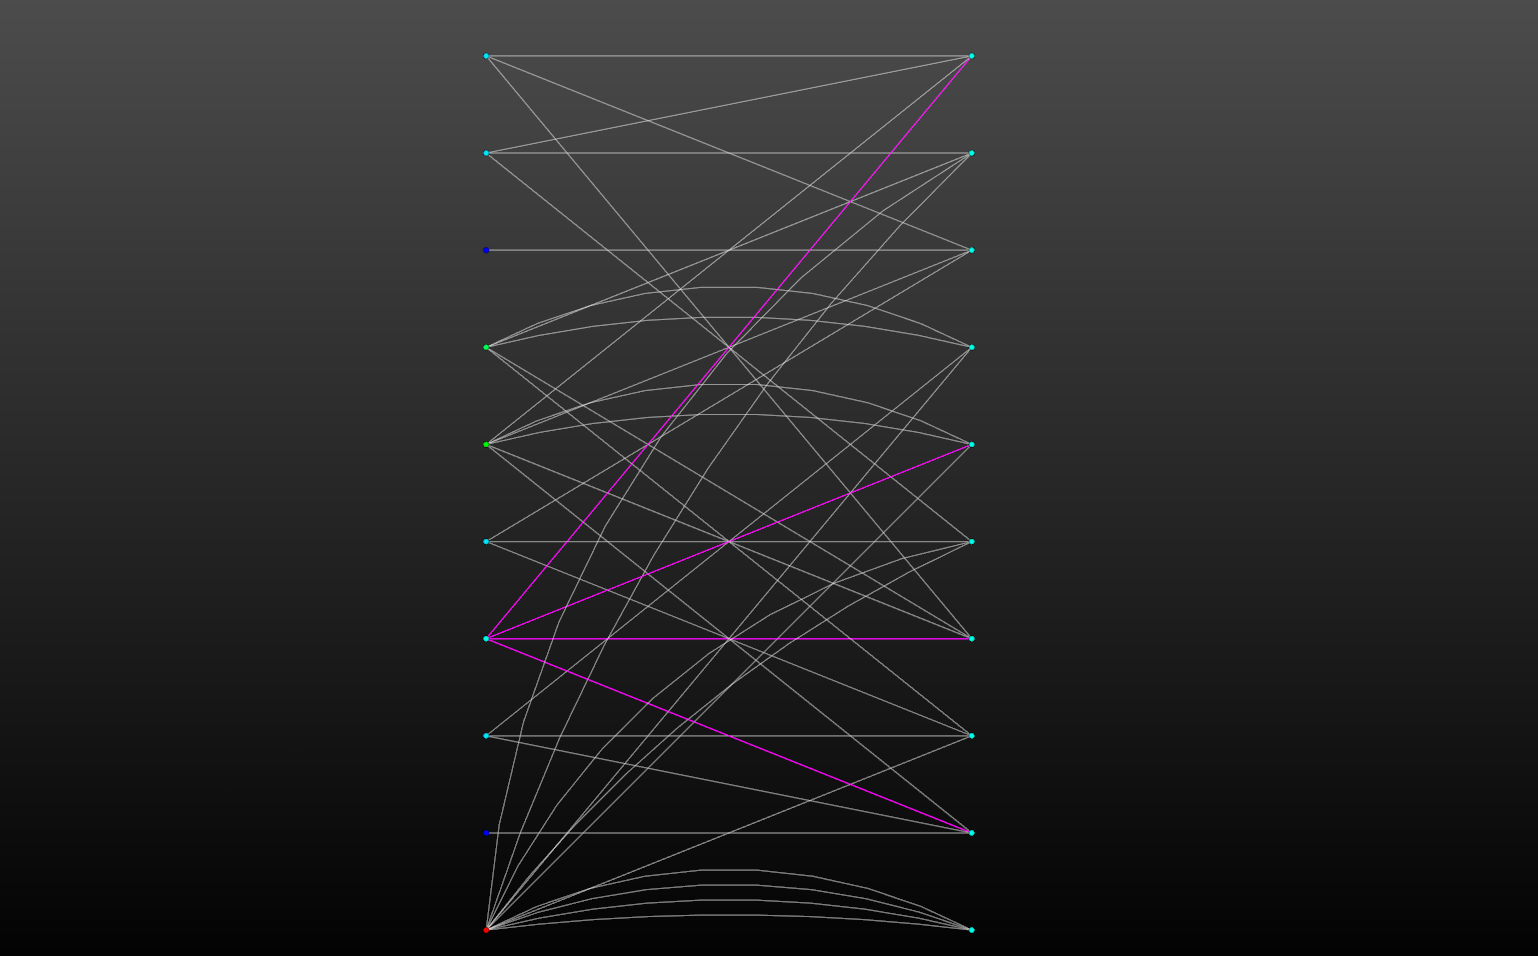
\includegraphics[width=\textwidth]{screen_shots/bipartite.png}
        \caption{A bipartite graph.}
    \end{figure}
    \begin{figure}[H]
        \centering
        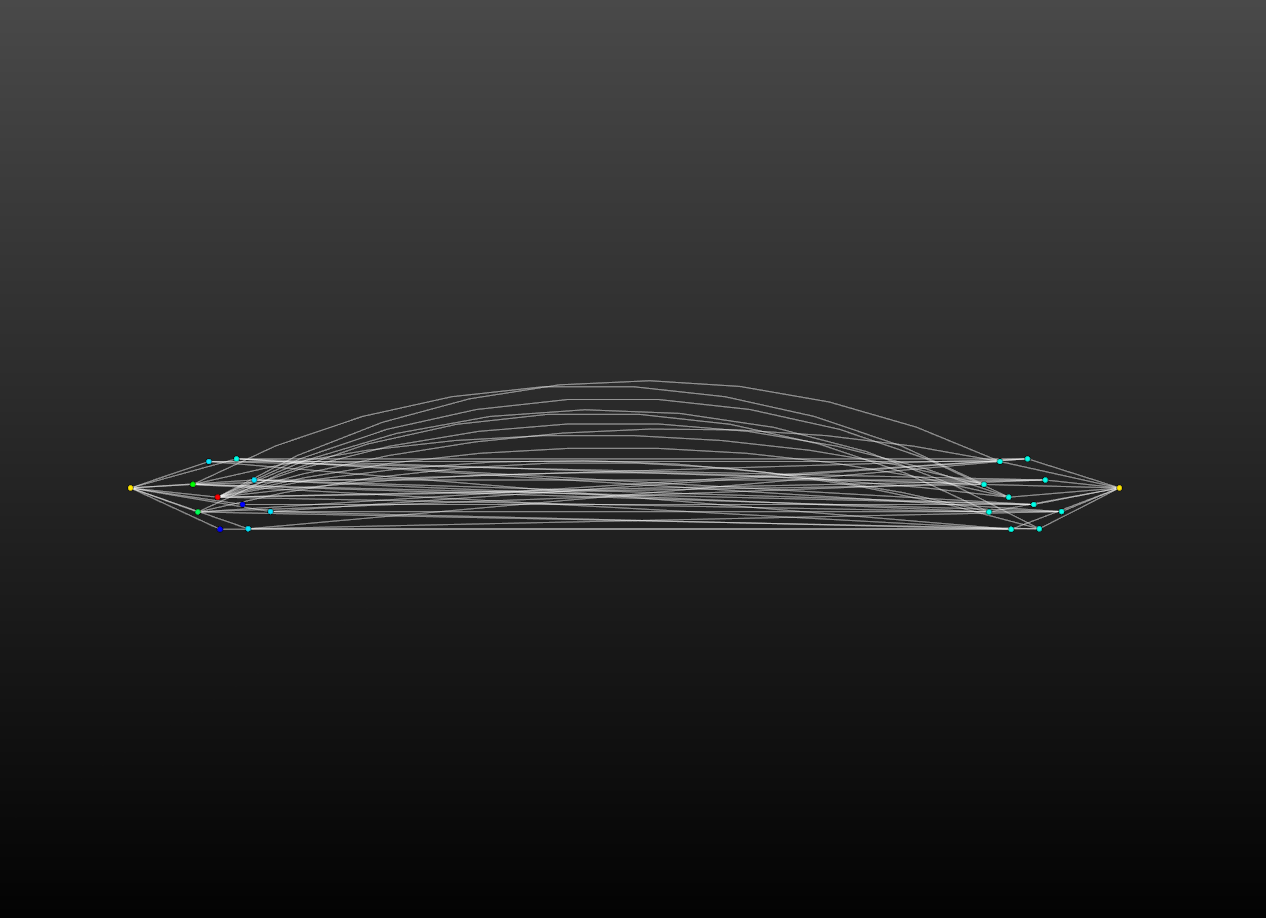
\includegraphics[width=\textwidth]{screen_shots/bipartite_cluster.png}
        \caption{A bipartite graph drawn with a clustering layout.}
    \end{figure}
    \begin{figure}[H]
        \centering
        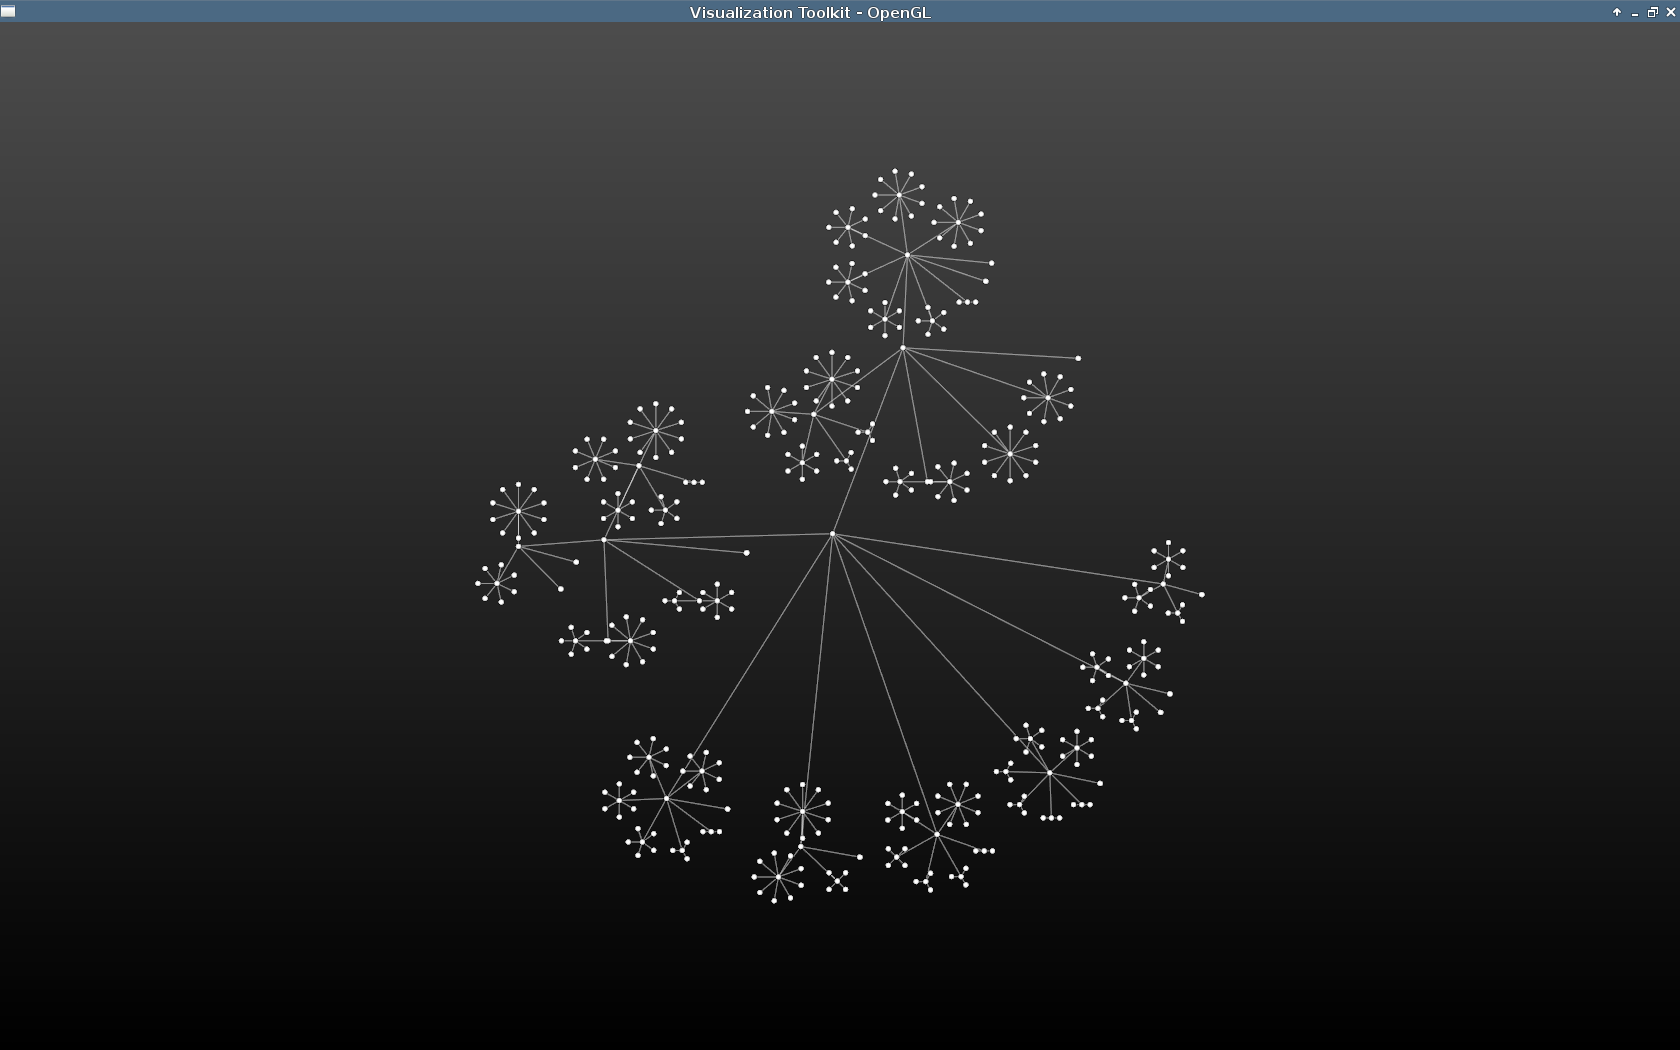
\includegraphics[width=\textwidth]{screen_shots/cosmic_tree.png}
        \caption{A tree drawn with the cosmic tree layout.}
    \end{figure}
    \begin{figure}[H]
        \centering
        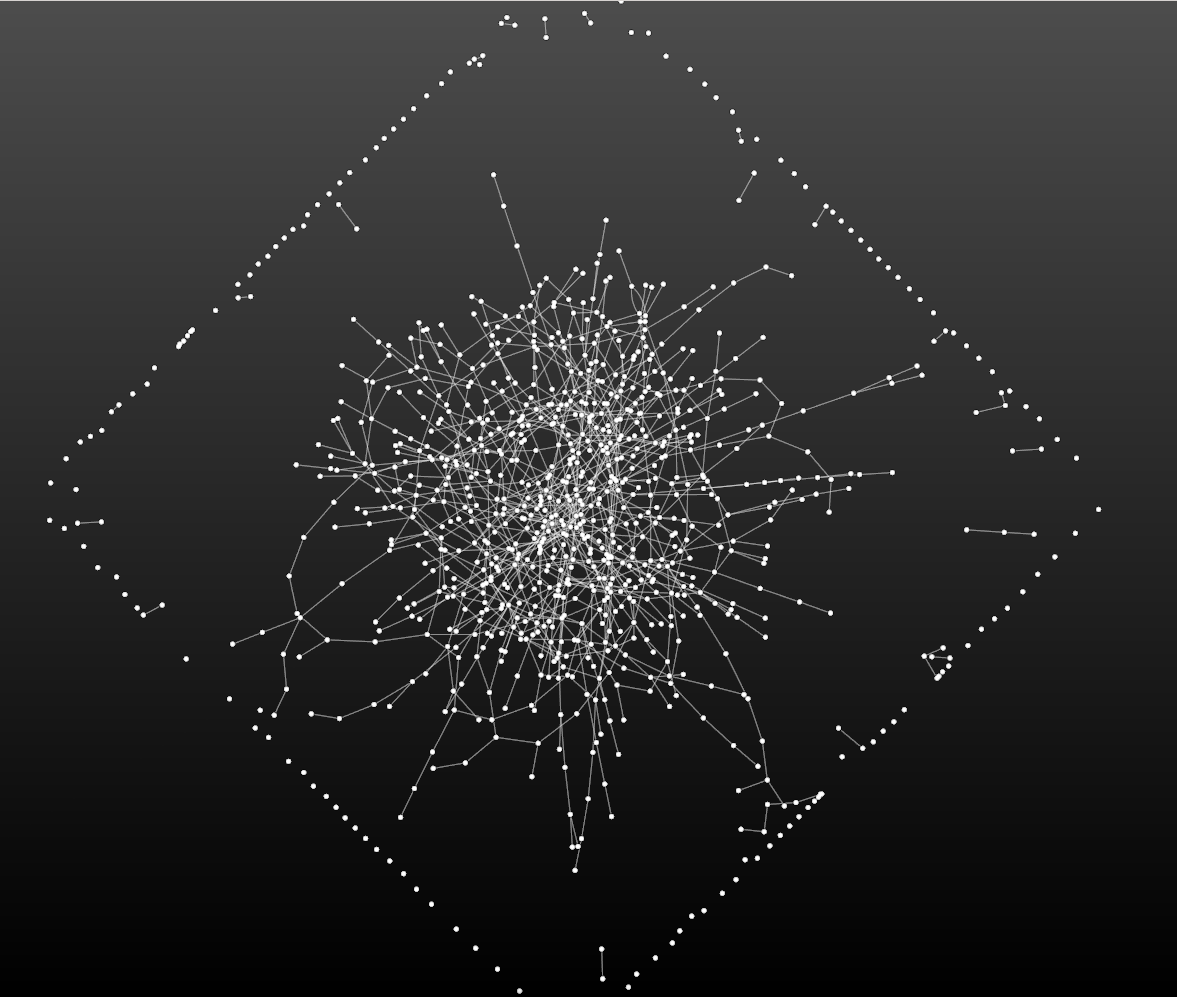
\includegraphics[width=0.5\textwidth]{screen_shots/disconnected.png}
        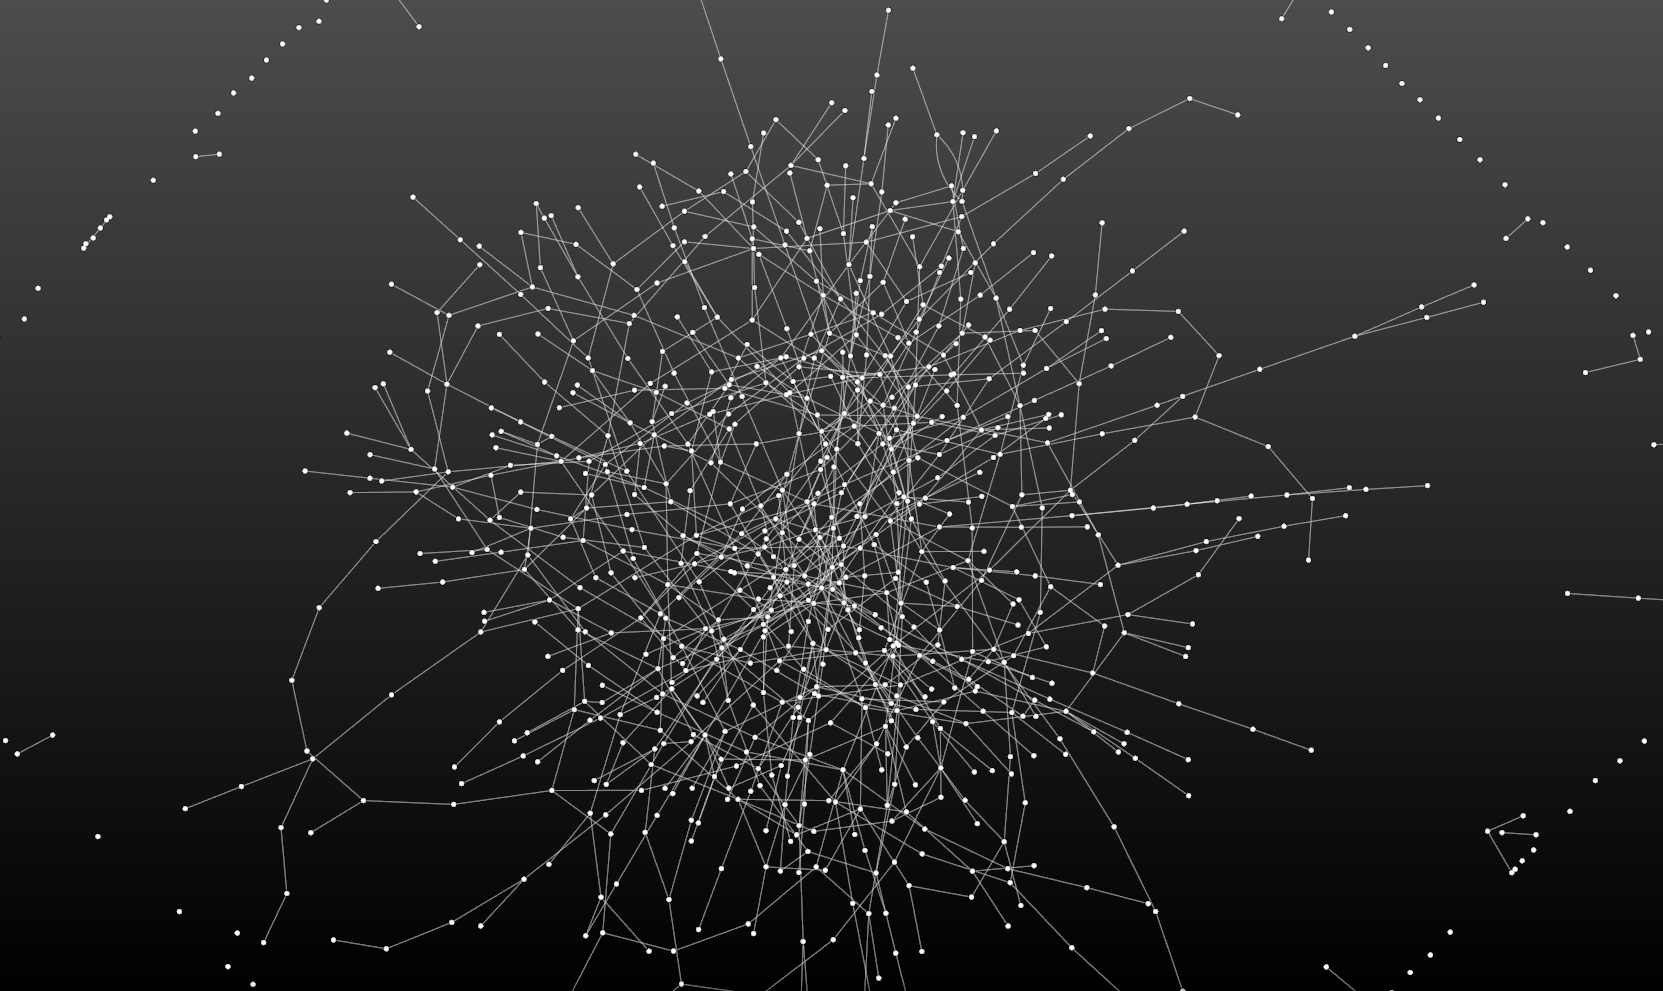
\includegraphics[width=0.5\textwidth]{screen_shots/disconnected_zoomed.png}
        \caption{A disconnected graph.}
    \end{figure}
    \begin{figure}[H]
        \centering
        \includegraphics[width=\textwidth]{screen_shots/tree.png}
        \caption{A tree.}
    \end{figure}
    \begin{figure}[H]
        \centering
        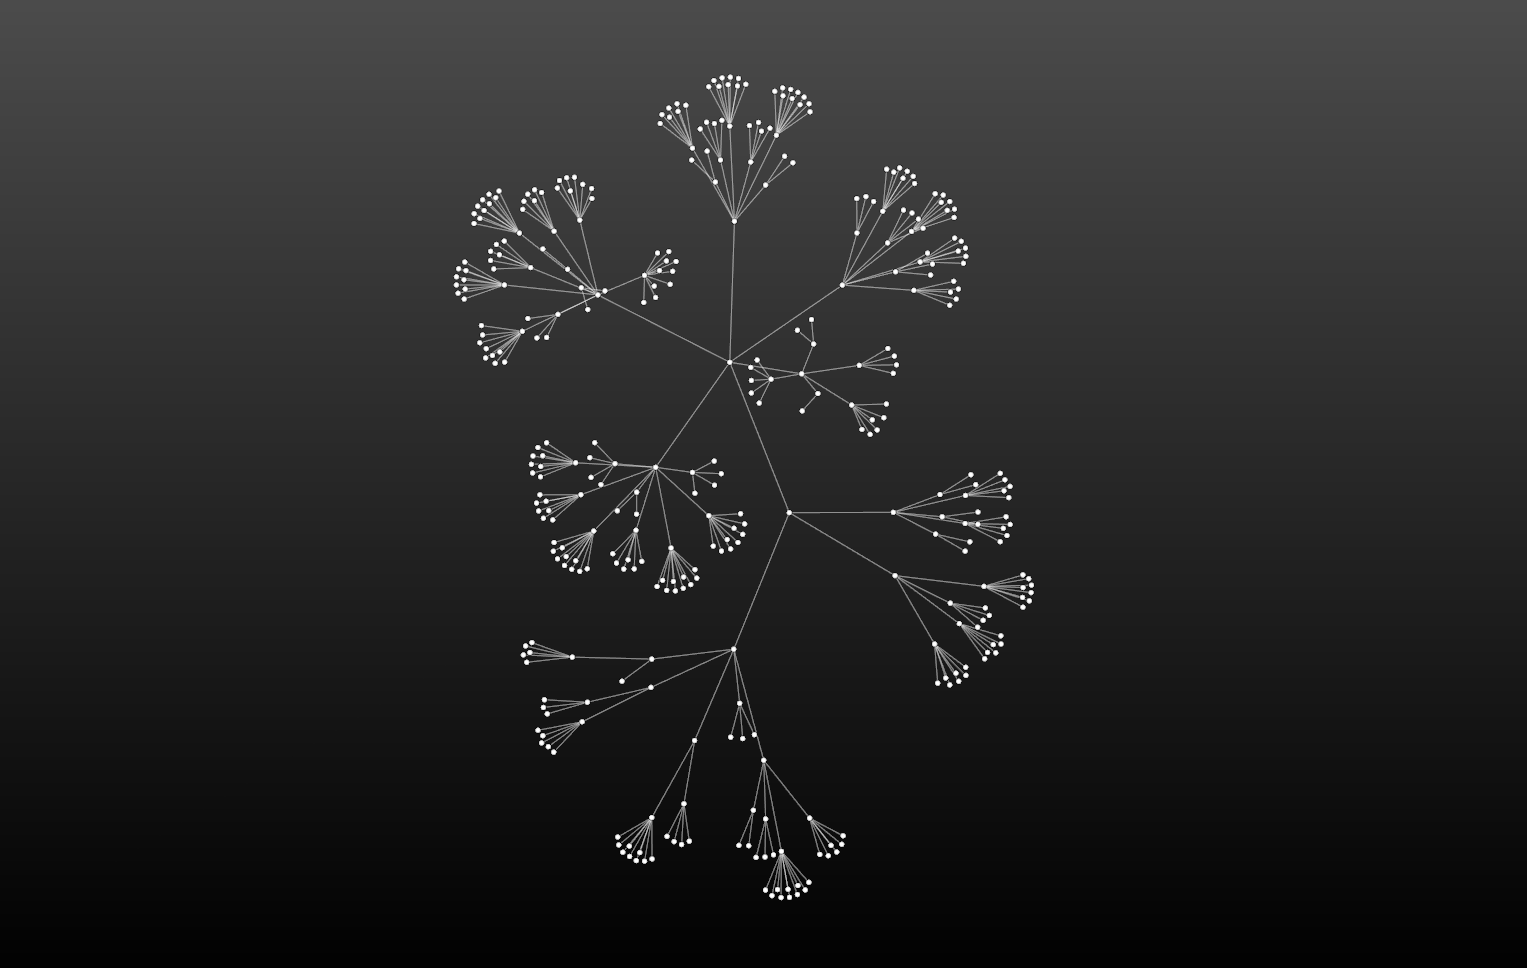
\includegraphics[width=\textwidth]{screen_shots/failed_tree.png}
        \caption{An alternate tree layout.}
    \end{figure}
    \begin{figure}[H]
        \centering
        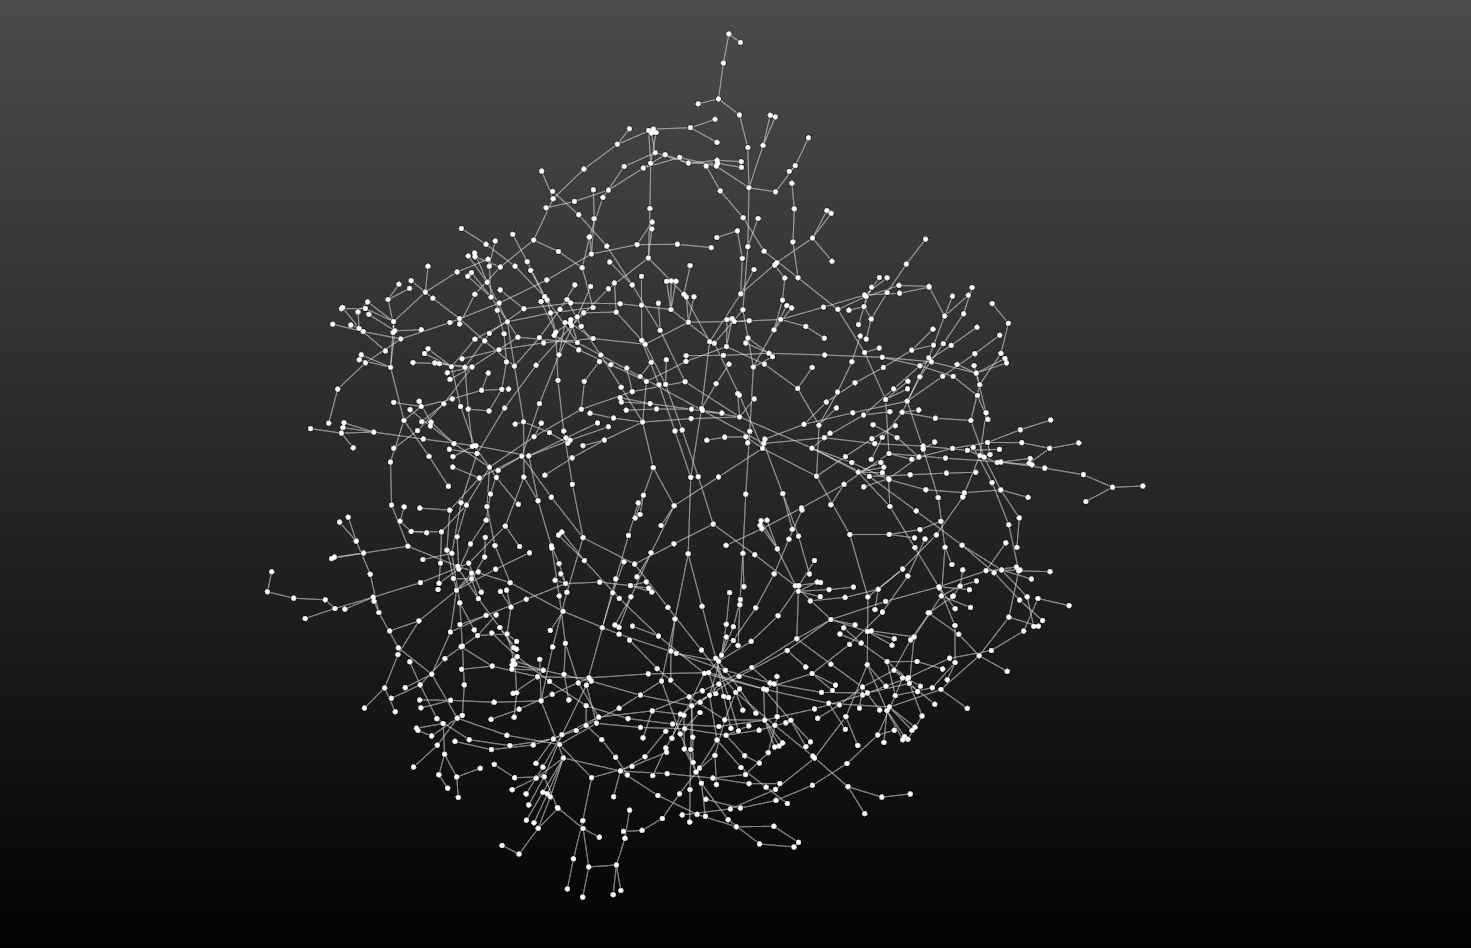
\includegraphics[width=0.5\textwidth]{screen_shots/non_planar.png}
        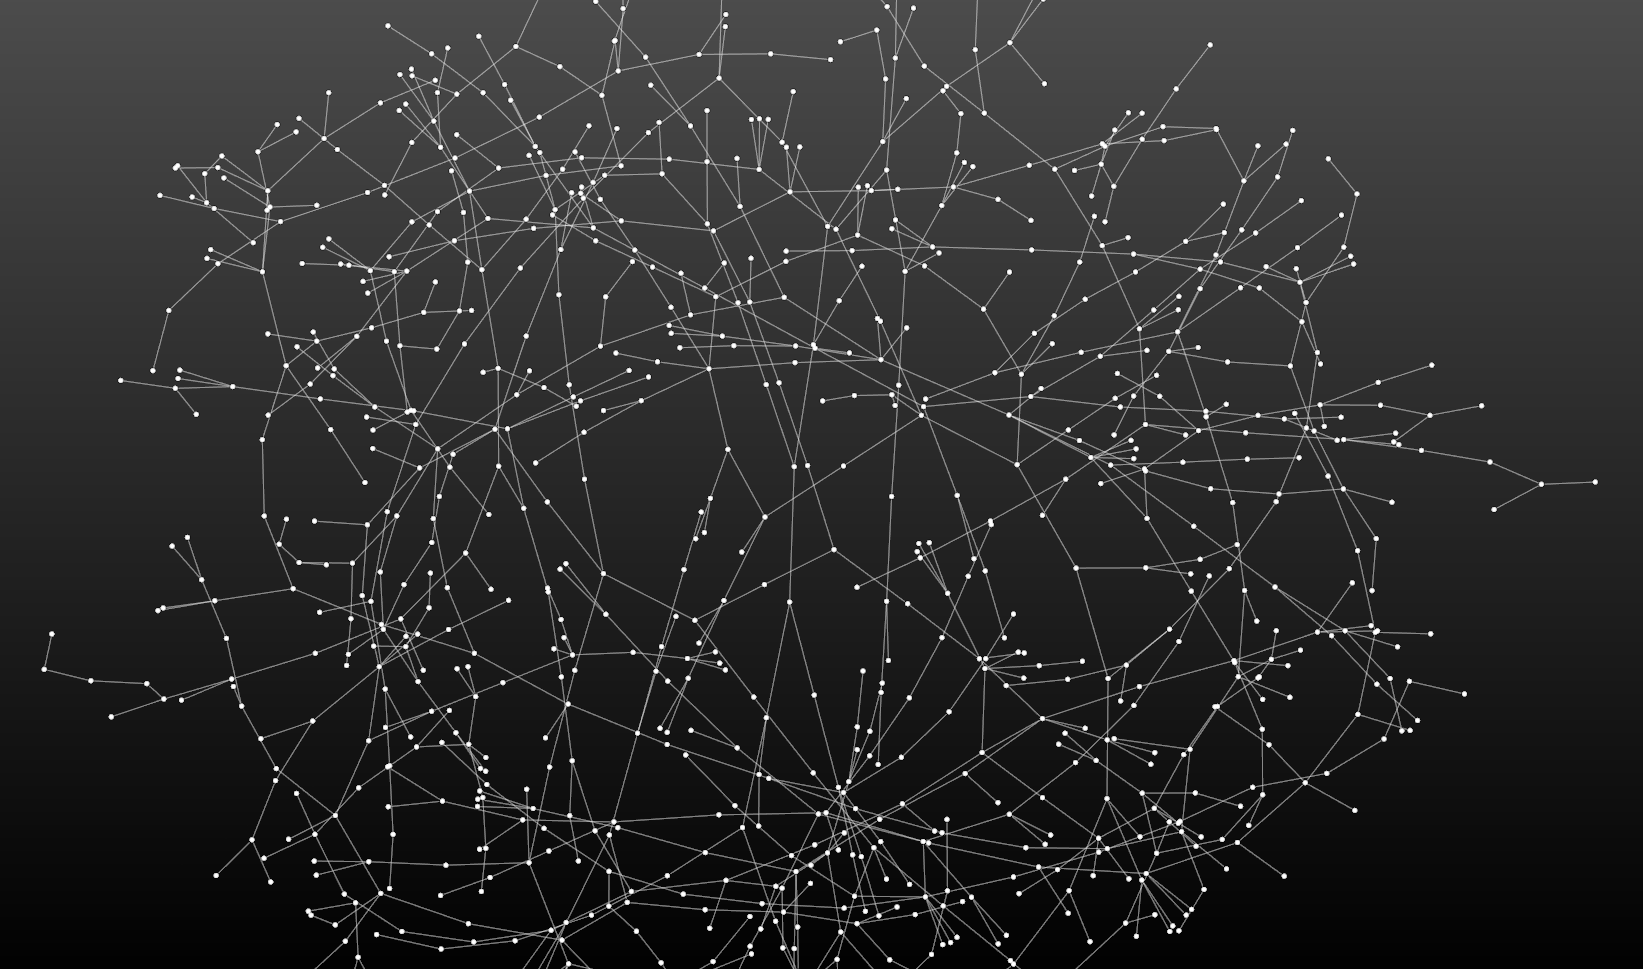
\includegraphics[width=0.5\textwidth]{screen_shots/non_planar_zoomed.png}
        \caption{A non planar graph.}
    \end{figure}
    \begin{figure}[H]
        \centering
        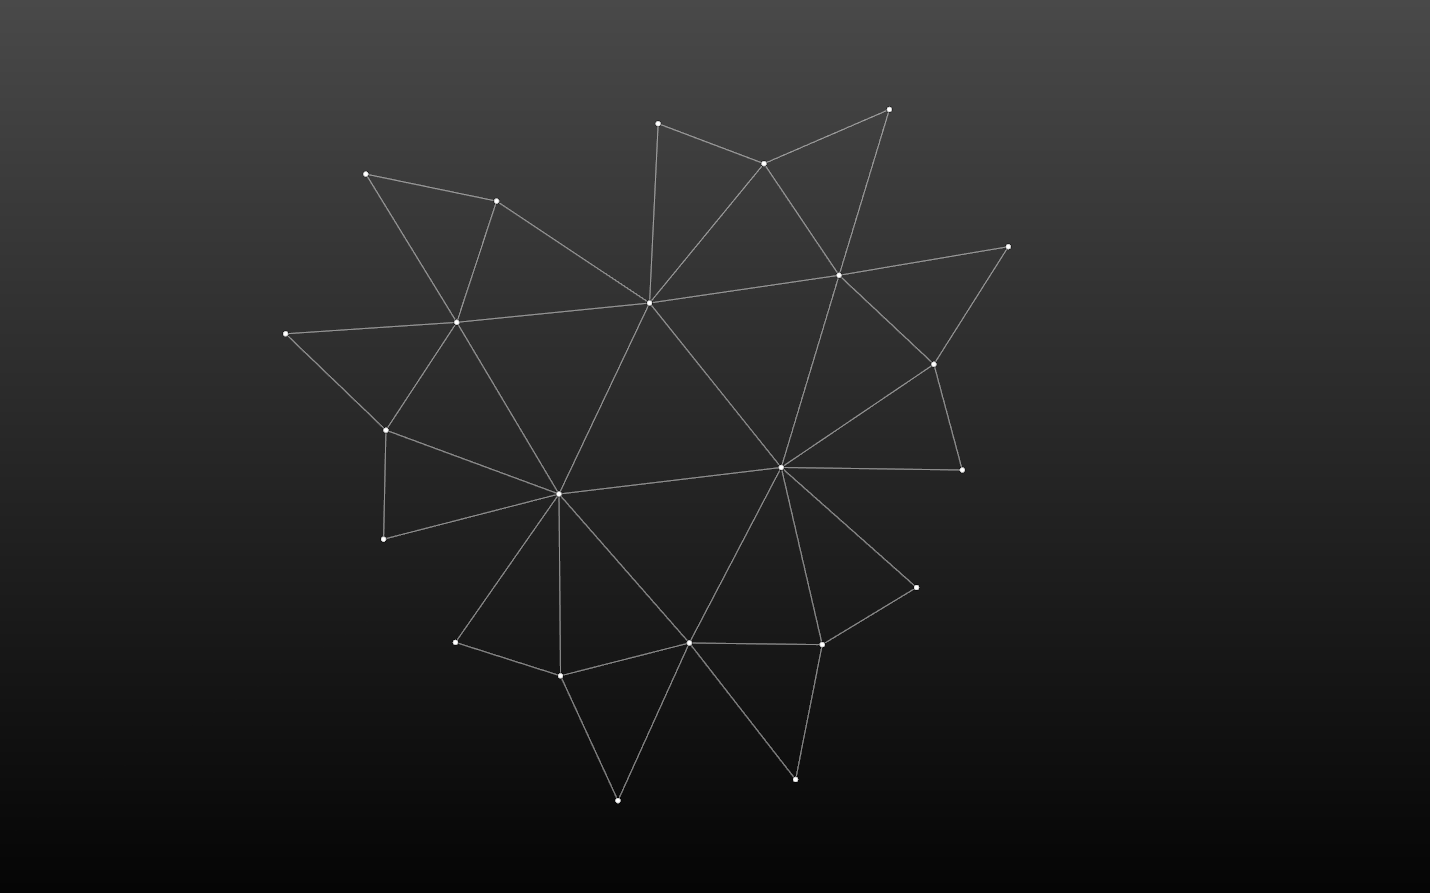
\includegraphics[width=\textwidth]{screen_shots/planar.png}
        \caption{A planar graph.}
    \end{figure}
\end{document}
